\documentclass{article}
\usepackage[utf8]{inputenc}
\usepackage{caption}
\usepackage{amsmath}
\usepackage{amssymb}
\usepackage{mathtools}
\usepackage{multicol}
\usepackage{graphicx}
\usepackage{wrapfig}
\usepackage{float}
\usepackage[makeroom]{cancel}
\usepackage{mhchem}
\usepackage{pst-plot}

\graphicspath{ {../images/} }

\renewcommand{\baselinestretch}{1.5} % line spacing
\newcommand{\fline}{\par\noindent\rule{\textwidth}{0.1pt}} % horizontal line (wide)

\title{Unit 3 Equilibrium\\Lesson 1 Equilibrium}
\author{Peter Zhang}

\begin{document}

\maketitle
\newpage
\tableofcontents
\newpage


% lesson 5
\section{Equilibrium}
Overview:\begin{enumerate}\item Types of Changes \item Equilibrium Law\item Free Energy\end{enumerate}

The reaction takes place at the \textbf{same rate} in the forward and reverse. BUT \textbf{NO net change}

\begin{figure}[H]
\centering
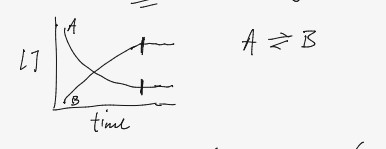
\includegraphics[width=\textwidth]{3.1figu1.jpg}
\captionof{figure}{The concentration as time passes}
\end{figure}

\pagebreak

\subsection{Dynamic Equilibrium}
This is a state of equilibrium where the rate of reaction from reactants to products and vice versa becomes the same, resulting in a net change of 0 in quantity of products and reactants. For instance, bromine in a closed system will establish a dynamic equilibrium between the liquid and gaseous phases. At a certain point, the equilibrium concentration of vapour is reached.

\begin{figure}[H]
\centering
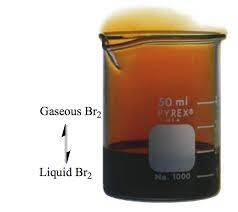
\includegraphics[width=200pt]{3.1bromine.jpg}
\captionof{figure}{System with bromine in liquid-gas equilibrium}
\end{figure}

\subsection{Equilibrium Initial/Reacting Properties}

\begin{itemize}
\item Can occur in both physical (change in state) + chemical reactions \\ basically \textbf{products and reactants and reactions occur at the same time}
\item Reactant [c] always starts at highest value \begin{itemize} \item [product] = 0 initially\item products then form until qiulibrium is reached\item called Dynamic Equilibrium\end{itemize}
\item Equilibrium can also be reqched from \textbf{either direction} (products can become reactants and vice versa)
\item All compounds do not need to have the same concentration
\end{itemize}

\subsection{Example with NaCl Dissolving in H2O}

The following dissolvation of \ce{NaCl2 in H2O} is an example of \textbf{HETEROGENEOUS EQUILIBRIUM AND SOLUBILITY}. 

A \textbf{saturated system in a closed system} will establish a dynamic equilibrium if there is excess solid present. Mixing Solid NaCl andwater will result in the solid dissolving.

\begin{figure}[H]
\centering
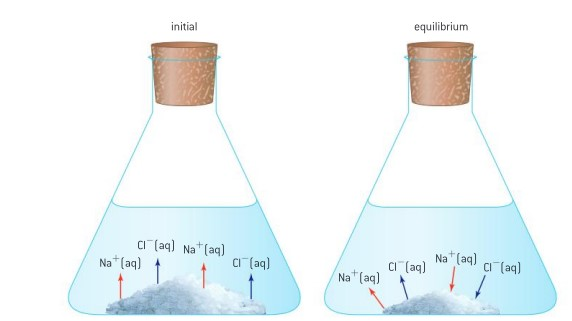
\includegraphics[width=200pt]{3.1fig2.jpg}
\captionof{figure}{A saturated solution is in dynamic equilibrium}
\end{figure}

In the figure above, there are 2 things we should take notice of:
\begin{itemize}
\item First: The NaCl is being hydrated and dissociated from its ionic compound. Basically, the ionic solid is dissolving.
\item Second: The \ce{Na+ and Cl- ions} precipitate8 back into its solid form, the \ce{NaCl} ionic compound.
\end{itemize}
Essentially, what happens is: \textbf{when the concentration of the NaCl solution reaches a certain point, the solution begins to reverse the reaction}.

\pagebreak

\section{Equilibrium Constant, $k_{c}$}
Just a value, \textbf{NO UNITS}. THIS SHOULD BE CALCULATED FOR THE FIRST EQUATION.

\begin{itemize}
\item $k_{c} >>$ 1 (very much greater) | favour products
\item $k_{c} <<$ 1 (very much less) | favour reactants
\item $k_{c} \approx $  1 (at equilib)
\end{itemize}

\begin{align*}
a\ce{A} + b\ce{B} &\ce{\rightleftharpoons} c\ce{C} + d\ce{D}\\
&= k_{c}\frac{[C]^{c}[D]^{d}}{[A]^{a}[B]^{b}}
\end{align*}

\section{Reaction Quotient, Q}
For a change in [] -- a change in concentration. If Q = $k_{c}$ reaction is at equilibrium. This means there is no observable change.

\begin{itemize}
\item $Q<k_{c}$ favours products
\item $Q>k_{c}$ favours reactants
\item $Q=k_{c}$ reaction is at equil
\end{itemize}

\subsection{Example}
Ex \ce{2H2 + O2 $\rightleftharpoons$ 2H2O}\ $k_{c} = 500$\\New Reaction: $[H_{2}]$ = 3.2M $[O_{2}]$ = 1.6M $[H_{2}O]$ = 7.4M.

$k_{c}$ only for initial reaction. If there are changes in the reaction, 

$$ Q = \ce{\frac{[H2O]^{2}}{[H2]^{2}[O2]}} = \ce{\frac{7.9^{2}}{3.2^{2}{1.6}}} = 3.34$$

The reaction favours the products because $Q < k_{c}$


% new page







\end{document}